\documentclass{beamer}
\usetheme{metropolis}
\usepackage{graphicx}
\usepackage{subfig}
\usepackage{tcolorbox}
\title{Calculus-Based Physics-2: Electricity, Magnetism, and Thermodynamics (PHYS180-02): Unit 1}
\author{Jordan Hanson}
\institute{Whittier College Department of Physics and Astronomy}

\begin{document}
\maketitle

\section{Unit 0 Review}

\begin{frame}{Unit 0 Review}
\textit{Physics} - $\phi\upsilon\sigma\iota\kappa\acute{\eta}$ - "phusik\'e": \textit{knowledge of nature} \\
from $\phi\acute{\upsilon}\sigma\iota\varsigma$ - "ph\'usis": \textit{nature}
\textbf{Reading: Chapters 1 and 2 (for Unit 1)}
\begin{enumerate}
\item Estimation/Approximation
\begin{itemize}
\item \alert{Estimating} the correct order of magnitude
\item \alert{Building} complex quantities
\item \alert{Unit analysis}
\end{itemize}
\item Review of concepts from Newtonian mechanics
\begin{itemize}
\item Kinematics and \alert{Newton's Laws}
\item Work-energy theorem, energy conservation
\item Momentum, conservation of momentum
\end{itemize}
\end{enumerate}
\end{frame}

\begin{frame}{Unit 0 Review}
Two molucules collide elastically.  Which of the following is true?
\begin{itemize}
\item A: Both potential energy and momentum are conserved for each molecule
\item B: Only the momentum is conserved for each molecule
\item C: Momentum and kinetic energy are conserved for each molecule
\item D: Neither momentum nor energy is conserved for each molecule
\end{itemize}
\end{frame}

\begin{frame}{Unit 0 Review}
Suppose a molecule is headed towards the wall of a container with speed $v$ and mass $m$.  If it collides elastically with the wall and returns in the exact same direction from which it came, what is the change in momentum of the molecule?
\begin{itemize}
\item A: $mv$
\item B: $\frac{1}{2}mv^2$
\item C: $mv^2$
\item D: $2mv$
\end{itemize}
\end{frame}

\begin{frame}{Unit 0 Review}
Do you remember how to take the derivative of an exponential function?  Let $f(t) = \exp(\alpha t)$.  What is $f'(t)$?
\begin{itemize}
\item A: $\exp(\alpha t)$
\item B: $\alpha\exp(\alpha t)$
\item C: $\exp(\alpha t)/\alpha$
\item D: $\exp(2\alpha t)$
\end{itemize}
\end{frame}

\begin{frame}{Unit 0 Review}
What about multiplying exponentials?  What is $f(t)g(t)$, if $f(t) = \exp(\alpha t)$ and $g(t) = \exp(\beta t)$?
\begin{itemize}
\item A: $\exp(\alpha\beta t)$
\item B: $\exp(\frac{\alpha}{\beta} t)$
\item C: $\exp(\frac{\beta}{\alpha} t)$
\item D: $\exp((\alpha+\beta) t)$
\end{itemize}
\end{frame}

\section{Unit 1 Summary}

\begin{frame}{Unit 1 Summary}
\textbf{Reading: Chapters 1 and 2}
\begin{enumerate}
\item Temperature, Heat, and the 0th Law of Thermodynamics
\item Heat flow and transfer mechanisms
\item Kinetic Theory of Gases
\end{enumerate}
\end{frame}

\section{JITT - Reading Quiz Results}

\section{Temperature, Heat, and the 0th Law of Thermodynamics}

\begin{frame}{Temperature, Heat, and the 0th Law of Thermodynamics}
\begin{figure}
\centering
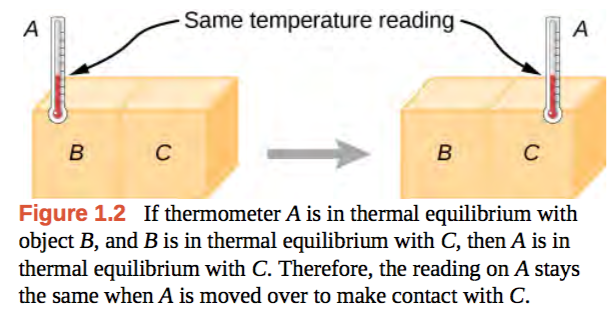
\includegraphics[width=0.9\textwidth,trim=0cm 4cm 0cm 0cm,clip=true]{figures/zero.png}
\caption{\label{fig:zero} The zeroeth law of thermodynamics.  We need this idea to have a firm understanding of temperature readings, because a \textbf{thermometer} is itself a thermal system.}
\end{figure}
\end{frame}

\begin{frame}{Temperature, Heat, and the 0th Law of Thermodynamics}
\begin{figure}
\centering
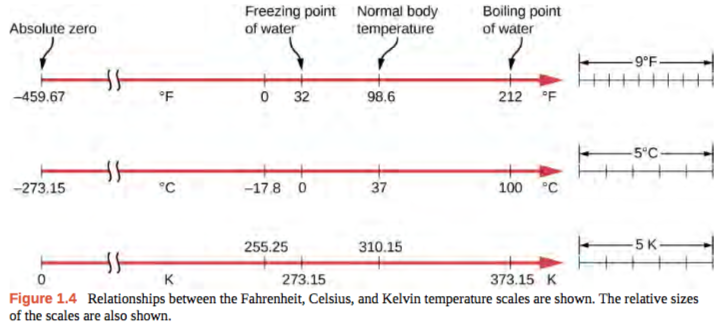
\includegraphics[width=0.95\textwidth,trim=0cm 1.5cm 0cm 0cm,clip=true]{figures/temp1.png}
\caption{\label{fig:temp1} Three temperature scales.}
\end{figure}
\end{frame}

\begin{frame}{Temperature, Heat, and the 0th Law of Thermodynamics}
\begin{figure}
\centering
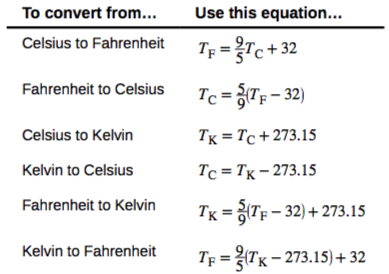
\includegraphics[width=0.7\textwidth]{figures/temp2.png}
\caption{\label{fig:temp2} Three temperature scales.}
\end{figure}
\end{frame}

\begin{frame}{Temperature, Heat, and the 0th Law of Thermodynamics}
Suppose the temperature of a system is raised by 10$^{\circ}$ F.  Which of the following is true?
\begin{itemize}
\item A: The increase is more than 10 degrees in $^{\circ}$C.
\item B: The increase is smaller than 10 degrees in $^{\circ}$C.
\item C: The increase is the same in $^{\circ}$C.
\item D: Depends on the initial temperature in $^{\circ}$F.
\end{itemize}
\end{frame}

\begin{frame}{Temperature, Heat, and the 0th Law of Thermodynamics}
Suppose the temperature of a system is raised by 10$^{\circ}$C.  Which of the following is true?
\begin{itemize}
\item A: The increase is more than 10 degrees in $^{\circ}$K.
\item B: The increase is smaller than 10 degrees in $^{\circ}$K.
\item C: The increase is the same in $^{\circ}$K.
\item D: Depends on the initial temperature in $^{\circ}$C.
\end{itemize}
\end{frame}

\begin{frame}{Temperature, Heat, and the 0th Law of Thermodynamics}
The formula for conversion from Celcius temperature to Fahrenheit temperatures is $T_{\rm F} = \frac{9}{5}T_{\rm C} + 32$.  Which of the following is true?
\begin{itemize}
\item A: $0^{\circ}-10^{\circ}$C is comparable to room temperature
\item B: $35^{\circ}-40^{\circ}$C is comparable to human body temperature
\item C: $30^{\circ}-35^{\circ}$C is comparable to human body temperature
\item D: $15^{\circ}-20^{\circ}$C outdoors would correspond to hot weather
\end{itemize}
\end{frame}

\begin{frame}{Temperature, Heat, and the 0th Law of Thermodynamics}
How do thermometers work?  What is temperature, really?  \textit{Temperature is a macroscopic indication of microscopic kinetic energy}.  We need the idea of \textbf{thermal expansion}: \\ 
\begin{equation}
\frac{dL}{dT} = \alpha L
\label{eq:linear}
\end{equation}
In Eq. \ref{eq:linear}, $T$ is the temperature, $L$ is the length of an object, and $\alpha$ is the coefficient of linear thermal expansion, in units of inverse degrees.
\end{frame}

\begin{frame}{Temperature, Heat, and the 0th Law of Thermodynamics}
\begin{figure}
\centering
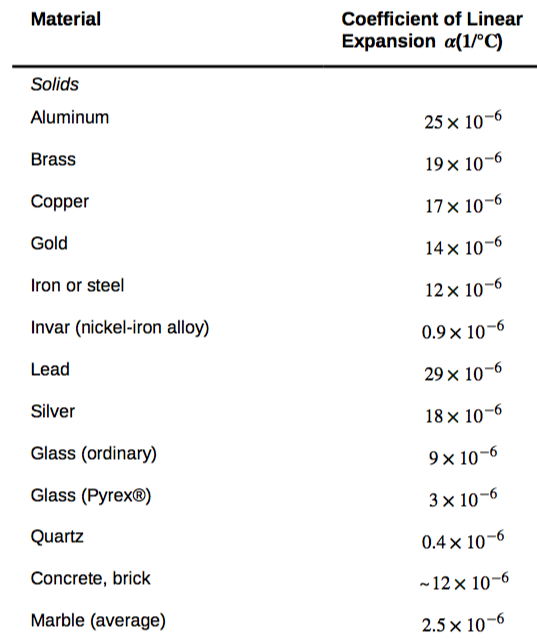
\includegraphics[width=0.55\textwidth]{figures/linear.png}
\caption{\label{fig:linear} Linear thermal expansion coefficients.}
\end{figure}
\end{frame}

\section{Conclusion}

\begin{frame}{Unit 1 Summary}
\textbf{Reading: Chapters 1 and 2}
\begin{enumerate}
\item Temperature, Heat, and the 0th Law of Thermodynamics
\item Heat flow and transfer mechanisms
\item Kinetic Theory of Gases
\end{enumerate}
\end{frame}

\section{Answers}

\begin{frame}{Answers}
\begin{columns}[T]
\begin{column}{0.5\textwidth}
\begin{itemize}
\item Momentum and kinetic energy are conserved for each molecule
\item $2mv$
\item $\alpha\exp(\alpha t)$
\item $\exp((\alpha+\beta) t)$
\item The increase is smaller than 10 degrees in $^{\circ}$C
\item The increase is the same in $^{\circ}$K
\item $35^{\circ}-40^{\circ}$C is comparable to human body temperature
\end{itemize}
\end{column}
\begin{column}{0.5\textwidth}
\begin{itemize}
\item ...
\end{itemize}
\end{column}
\end{columns}
\end{frame}

\end{document}
